	Mechanisms for coping with food crises include direct provision of food aid \citep{timmer2010reflections}. However this international aid needs to be directed. Many times the most affected regions are not proximal to the climate event but geographically separated.\par


In chapter \ref{relatedWorkChapter} a literature study is conducted with a high-level summarization of related works. In chapter \ref{foodTradeNetworkChapter} an introduction to the international food trade network is given. Chapter \ref{networkAnalysisChapter} analyses the international food trade network with respect to network graph theory. Chapter \ref{effectiveVisualizationsChapter} emphasizes properties of effective visualizations that led to the design of the dashboard. Chapter \ref{systemChapter} illustrates the system architecture. The Chinese drought is explored as a case study with the tool in chapter \ref{caseStudyChapter}. Finally chapter \ref{conclusionsChapter} summarizes this work.

\section{Indicators of Vulnerability}

\subsection{Food Security}
\subsubsection{Food Availability}
National average DES (dietary energy supply). FAO defined minimum dietary energy requirement (MDER) (1844 kcal/cap/day) and average dietary energy requirement (ADER) (2353 kcal/cap/d) for the period of 2014-2016.
Two ways to obtain: a) domestic production and b) benefit from food trade, either from income of food exports or import of external resources. \cite{porkka2013food}
\subsubsection{Food Self-Sufficiency}
Dietary energy production (DEP) compared to global ADER
Low production: DEP of less than 2000 kcal/cap/d
Insufficient production: DEP of 2000–2500 kcal/cap/d
Sufficient production: DEP of 2500–3000 kcal/cap/d
High production: DEP of over 3000 kcal/cap/d \cite{porkka2013food}
How to change: Average value of food production -> DEP
Low self-sufficiency + (high export single good?)
\subsubsection{Food Trade}
High net imports: DES – DEP of over 1500 kcal/cap/d
Moderate net imports: DES – DEP of 500–1500 kcal/cap/d
Low net imports: DES – DEP of 0–500 kcal/cap/d
Low net exports: DEP – DES of 0–500 kcal/cap/d
Moderate net exports: DEP – DES of 500–1500 kcal/cap/d
High net exports: DEP – DES of over 1500 kcal/cap/d \cite{porkka2013food}
\subsubsection{Composition of Diet}
Average supply of protein of animal origin: Food\_Security\_Indicators.xlsx

\subsection{Climate Change Vulnerability Indicators}
Enumerate these more better.
\subsubsection{Indicator 1}
\subsubsection{Indicator 2}
\subsubsection{Indicator 3}

\subsection{Agricultural Vulnerability to Climate Change}
Introduce composite index methods and assessment of each with \cite{wirehn2015assessment}.
\section{VISUALIZATION}
\subsection{Geospatial}
Why use geospatial?
\subsection{Network}
How to incorporate nodes/edges in geospatial effectively.
Motif simplification. \cite{dunne2013motif}
\subsection{Chloropleth v. Size of Nodes}
Or some other way to indicate a relative value.
\subsection{Effectiveness}
Using information from \cite{preston2011putting} defend why this is an effective method for displaying the data.



This general question can be split into several sub-questions, which are listed below.\par
Research questions:
\begin{itemize}
	\item Which “climate singularities” have an impact on the agricultural trade network? Is the impact limited to droughts or are there other relevant atmospheric events?
	\item How far-reaching is the impact of each of these climate singularities, if it appears in a specific region of the world? The import and export of which countries (= nodes of a weighted graph) will be impacted, and to which extent?
	\item How can such singularities and their impact be projected to the future, using statistical modelling?
	\item How can integrated climate and agricultural trade data be visualized, and how does this visualization facilitate the ongoing analysis?	
\end{itemize}\par
\section{Research Plan}
\begin{enumerate}
	\item Literature review
	\begin{itemize}
		\item World trade networks
		\item Climate change*
		\item Algorithms for weighted graphs*
		\item Geospatial network visualization
		\item Time series analysis and modeling*
	\end{itemize}
	\item Determine research methodology concerning graph algorithms and statistical modelling
	\begin{itemize}
		\item How to find “climate singularities”?
		\item How to correlate these singularities with the agricultural trade network? Spatial and temporal correlation techniques? Combination?
	\end{itemize}
	\item Implement methods in connection with geospatial visualization:
	\begin{itemize}
		\item Setup of a visualization platform
		\item Integration of relevant data sets
		\item Interaction features
	\end{itemize}
	\item Analysis together with domain-experts (Shade Shutters)
\end{enumerate}
\section{Background and Motivation}




Coupled with fiscal instability of importing countries and a higher percentage of poor, trade dependencies are an area of concern. 



The need to recognize a developing pattern in order to mitigate two-tier pricing is emphasized.

This also means that the 

However this trend does have its risks. Major exporters are capable of causing larger supply shocks. 





In the context of this thesis those supply shocks are represented as disruptions to trade links in the network graph. 

These supply shocks are essentially what the modeling is representing.

\cite{porkka2013food} the growing international dependence on trade as a means of meeting growing caloric needs.



Self-sufficiency is correlated to a country's water resources and trade dependency is a result of insufficiency. 







\section{International Food Trade Network}
There is an increasing dependency on trade to feed the world \citep{d2014feeding}, resulting in the potential for regional production declines to be felt globally. Their work highlights the food trade network's role in food security. Disruptions to the food trade network can directly effect food security. Food security in a country is a function of national production and international trade.\par

This is represented in a network graph as a small weight of in-degree edges.

Diversified import portfolios can mitigate the source of supply problems \citep{silberglitt2015critical}. If there is to be a large volume of incoming trade, the quantity of links should be high to meet this need. This would minimize the associated issues including price spikes or volatility.   Distribution of the global food supply, including the international food trade network, could be improved to increase food security worldwide. Food security can, in part, be solved by the food trade network. A diversified import portfolio can be important for securing food supply \citep{fader2013spatial}. Some countries rely heavily on imports to sustain feed their people.    As these studies show countries are becoming more import-dependent. This visual analytics system focuses on the climate events effect on these import trade links, the supply shocks.\par




Gross domestic product (GDP) is important in determining whether there exists a trade link between two countries. This is because countries with large relative GDPs tend to be linked to many with small GDPs. Countries with many trade partners are on average connected to countries with few partners. Partners of well-connected countries are less interconnected than those of poorly connected ones.





The paper goes on to display how financial crises can be explained by the topology of the international trade network. 
















introduce a concept of reciprocity in simplifying the network graphs with respect to imports and exports.  \citep{zhou2016structure} provides a hierarchical structure consisting of four tiers that correlate with network centrality.  The same is true when it comes to the world trade network.  In the international food trade network there is a high betweenness of a small number of countries that are the major food exporters \citep{garlaschelli2005structure}.   Historical analysis of certain players in the international trade network suggest the importance of positioning in the network to affluence. This paper implies a temporal change in network structure confirming other research on increasingly trade dependent food sources. The rise in network density implies a larger number of trade partners, though the density index is still low enough to maintain incompleteness in the network. \cite{serrano2003topology} offer statistics on the topology of the world trade network. The importance of the properties of in and out degree distributions are emphasized. The distributions deviate significantly from a randomized network suggesting self-organization. The scale-free nature and hierarchical architecture are guided by this self-organization of the network.  These topological attributes are the basis for \par






In order to accurately identify the cascading effects of a climate event, understand the food trade network, its topology and composition, to .\par
To this end previous literature on the international food trade network is reviewed. Given that the food trade network can be naturally represented as a network graph, previous work related to network graphs is also reviewed. Current visualizations and techniques are reviewed to ensure efficacy in presentation.\par
Current visualizations have focused on displaying the food security indices based on global climate models. While these models are useful for long-term forecasting and prediction they do not aid in the reaction to single catastrophic climate events. Other visualizations have only considered subsets of the food trade network.






This provides the human computer interaction foundational tasks for this visual analytics paradigm. 





Interactivity can aid in the analysis step in the visual analytics paradigm. 



Given the nature of the international food trade network and the number of edges present





A zoomed out view is usually the initial overview strategy which provides the basis for a visual analytics dashboard. The main visualizations in the dashboard include a network graph and a geospatial map.\par

In information visualizations analytic reasoning can be done at two different points; primarily by human analysts or primarily computational. This lends itself to two different types of visual interactions; one where the pieces are manipulated by the user and one where the computational methods are manipulated by the user \citep{andrienko2011challenging}. In this system the majority of interactions are manipulated by the user. \cite{keim2008visual} defines visual analytics as combining automated analysis techniques with interactive visualizations for an effective understanding, reasoning and decision making on the basis of very large and complex data sets. The inclusion of prediction choropleth on the cartographic map helps transform the information visualization into a visual analytics tool. By aiding the user in making correlations we allow for decision support. Allowing for filtering helps maintain the feedback loop \citep{keim2008visual} in which the user can make a decision.\par

There are a number of ways to minimize edge crossing. One method is by edge compression, reducing the number of edges.   This is in contrast to the node and edge aggregation of motif constriction. 




In the context of network graph visualization  Aesthetic rules are constraints in practice for drawing network graphs. These rules include even distribution of nodes and edges, sub-structure uniformity and minimization of edge crossings.








As with my dashboard \cite{henry2007nodetrix} is attempting to visualize another large and complex network, social networks. The result is a hybrid visualization of the two popular representations, adjacency matrices and network graphs. Adjacency matrices are used in communities, acting as nodes in a traditional graph. The links residing between matrices visualize the overall structure of the network.


\cite{van2016reducing} suggests that network evolution is important if we are going to be visualizing current and potential futures states. There are two different basic approaches: time to time and time to space. A key point in creating an effective representation is a balance between fewer images lacking temporal data and many images lacking interpret-ability.\par

The geospatial map offers its own unique challenges. \cite{andrienko2011challenging} also identifies potential areas of concern when utilizing geospatial data.
\cite{preston2011putting} offers pros and cons of directly visualizing climate change indicators and risk on a geographical map. We use this information to offer up multiple coinciding visualizations in order to mitigate the potential bias of a single visualization.







Visual analytics is defined by \cite{cook2005illuminating} as "analytical reasoning facilitated by interactive visual interfaces." It has become the preferred tool for domain-experts exploring large data sets.
This visual analytics dashboard uses the mantra defined by \cite{shneiderman1996eyes}: overview first, zoom and filter, then details-on-demand.

\begin{figure}[htb]
	\center{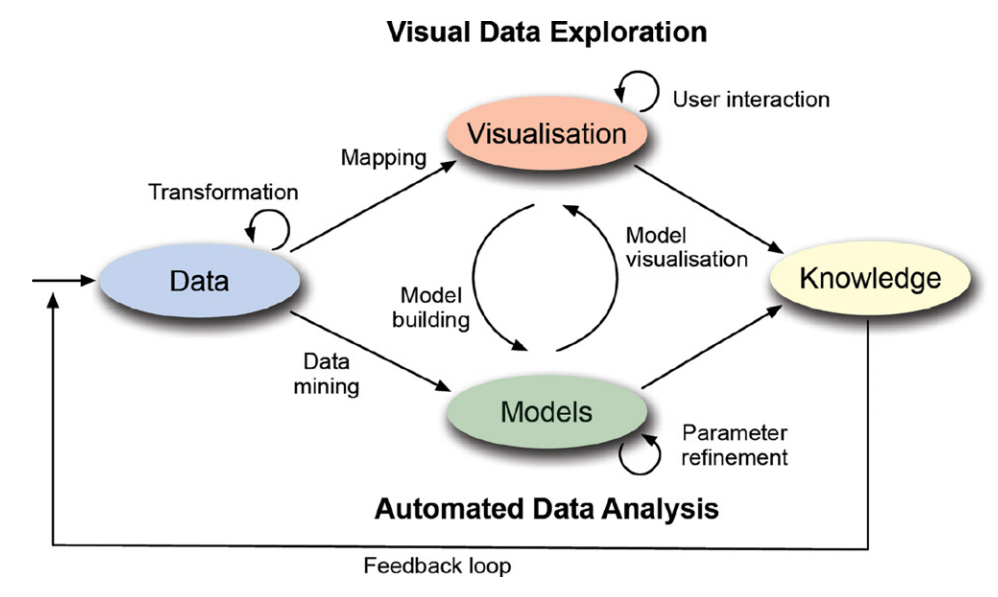
\includegraphics[width=\textwidth]{figures/keim.png}}
	\caption{Visual Analytics Framework, \citep{keim2008visual}}
	\label{keim}
\end{figure}

Visualizing a network graph can be done in two primary ways: node-link diagrams and adjacency matrices. The most familiar visualization is the node-link diagram . \cite{ghoniem2004comparison} considers the two different representation and compares the readability of the two graphs. Although the international trade network starts out with a large number of nodes, when filtering is applied \citep{shneiderman1996eyes} it has a limited number of nodes. Therefore when choosing the appropriate visualization I consider it a small graph, and node-link diagrams are more readable \citep{ghoniem2004comparison}.\par
Node placement is a consideration when network visualization is concerned. A common layout strategy is based on geographic representation \citep{shneiderman2006network}. This geographically representative positioning is used in both of the main visual representations. The linked multiple views of the familiar world map (choropleth) and the network visualization allow for a greater understanding \citep{rodgers2005graph}.\par
When visualizing a network minimizing edge crossing is the most important aesthetic consideration \citep{purchase1997aesthetic} for improving human comprehension. A number of different algorithms for graph visualization were reviewed (\cite{herman2000graph}, \cite{dunne2013motif}, \cite{holten2009force}) that help with this consideration. \cite{herman2000graph} overviews a number of basic graph layout algorithms in the context of information visualization. \cite{dunne2013motif} offers a technique to simplify highly clustered network graphs by aggregating subnetworks. Simplifying the drawing of certain types of motifs can greatly increase readability in dense network graphs. \cite{holten2009force} shows another example of a technique aimed at simplifying complex network graphs. This is achieved by bundling of similarly drawn edges and subsequent splitting of the edges closer to the termination node. Ultimately these algorithms were removed from consideration in favor of mental mapping \citep{eades1991preserving}. Nodes were positioned approximately geographic to aid in the establishment of this mental map. The minimization of edge crossing is accomplished interactively by dragging of nodes after a simulation baseline is established.\par
Effective human computer interaction is an important piece in any visual analytics system. The network visualization is a overview representation of the food trade network. Zooming and filtering is accomplished with uniform scaling in order to preserve the mental map \citep{eades1991preserving}.



Visualization is only only one part of a visual analytics system, knowledge is the end goal. \cite{keim2008visual} states the challenge is to identify the best automated algorithm for the analysis task at hand, identify its limits which can not be further automated, and then develop a tightly integrated solution with adequately integrates the best automated analysis algorithms with appropriate visualization and interaction techniques\par




Effective human computer interaction is an important piece in any visual analytics system. The network visualization is a overview representation of the food trade network. Zooming and filtering is accomplished with uniform scaling in order to preserve the mental map \citep{eades1991preserving}.



Visualization is only only one part of a visual analytics system, knowledge is the end goal. \cite{keim2008visual} states the challenge is to identify the best automated algorithm for the analysis task at hand, identify its limits which can not be further automated, and then develop a tightly integrated solution with adequately integrates the best automated analysis algorithms with appropriate visualization and interaction techniques\par













	After identifying a country and trade good exploration will continue further with the geospatial, line graph and network graph visualizations to determine the extent of the trade network impact for this particular parameter selection. After executing a simulation users are able to immediately see the downstream secondary and tertiary effects on the trade network. Actual trade link effects (network graph link size changes), triadic significance profile deviations (line graph) and vulnerability measures (choropleth) are available as a visualization in the dashboard. Through the feedback loop \citep{keim2006challenges} the results are refined by consecutive iterations.\par



	A base vulnerability index (choropleth) is provided to the user and domain-experts can make further determinations as to the vulnerability of the identified country based on other factors such as governance or economic health of the country that is outside the scope of this thesis. The model can then be manipulated to further explore if a climate singularity would have a measurable impact on the world agricultural trade network. Using data and previous research domain-experts will be able determine a subset of agricultural goods and countries which are vulnerable to a particular climate event based on these predictions.\par
